% Created 2025-09-13 Sat 15:18
% Intended LaTeX compiler: pdflatex
\documentclass[11pt]{article}
\usepackage[utf8]{inputenc}
\usepackage[T1]{fontenc}
\usepackage{graphicx}
\usepackage{longtable}
\usepackage{wrapfig}
\usepackage{rotating}
\usepackage[normalem]{ulem}
\usepackage{amsmath}
\usepackage{amssymb}
\usepackage{capt-of}
\usepackage{hyperref}
\author{Jackson Mowry}
\date{Sat Sep 13 11:26:11 2025}
\title{Hash Attack Project Report}
\hypersetup{
 pdfauthor={Jackson Mowry},
 pdftitle={Hash Attack Project Report},
 pdfkeywords={},
 pdfsubject={},
 pdfcreator={Emacs 30.2 (Org mode 9.7.11)}, 
 pdflang={English}}
\begin{document}

\maketitle
\section*{Hash Attack Basics}
\label{sec:org6702e67}
In this project we're performing two different types of attacks against the SHA-1 cryptographic hashing function. The first is a second preimage attack, which is defined by first selecting a hash digest and then attempting to find another input that produces the same output. This type of attack is protected by the ``weak-collision'' resistance property of cryptographic hashing functions. The second type attack is a collision attack, in which attackers attempt to find any 2 messages (that are not equal) that produce the same output.

The former is a much harder task as we are essentially required to cover the entire search space in order to find a collision. On the other hand, a collision attack is a much easier problem because we can continue to generate hashes, while comparing them against all previously generated hashes. For this reason we will see large differences in the number of iterations necessary to produce a collision.
\section*{Methods}
\label{sec:org39cccf1}
For this project I chose to write my driver code in C, utilizing that small SHA-1 C library from \texttt{halloweeks}. In order to speed up the expected time for calculating collisions I utilized multi threading. Truncated hashes were stored within a 32-bit integer (truncated length ranged from 8-22 bits), allowing for much quicker comparison.
\subsection*{Second Preimage Attack}
\label{sec:orgb4598ff}
For the preimage attack I grabbed 160 bytes of random data from \texttt{/dev/urandom}, hashed, and finally truncated it to the desired bit length. This desired hash was then broadcast to each worker thread who gather 160 bytes of random data and repeated the same process until a collision was found. At the end the total number of iterations across all threads was totaled and reported.
\subsection*{Collision Attack}
\label{sec:org45eee9c}
The collision attack was slightly more complicated as each thread would need to communicate with all other threads on the hashes it had already calculated. For this I used a lock free list data structure that allowed threads to add their calculated hashes one at a time without waiting on other threads. This was made safe by the fact that each thread would first look at the length of the list (an atomic size\textsubscript{t}) and check its hash against all other hashes less than that length. Only when the thread was done with this process would it increment the number and add its value to the list. With this in place a thread would not be concerned with values that were added after it began looking at the list, saving the need for a lock around the data structure.

Once again, when a collision was found the total number of iterations (the length of the list) was reported.
\section*{Second Preimage Attack}
\label{sec:org96aff78}
In a second preimage attack the attackers have already defined or selected a target digest, the goal is to then find another input that can produce that output. If hashing a specific input does not yield a match they simply need to move on to the next input, discarding the work done already.

\begin{center}
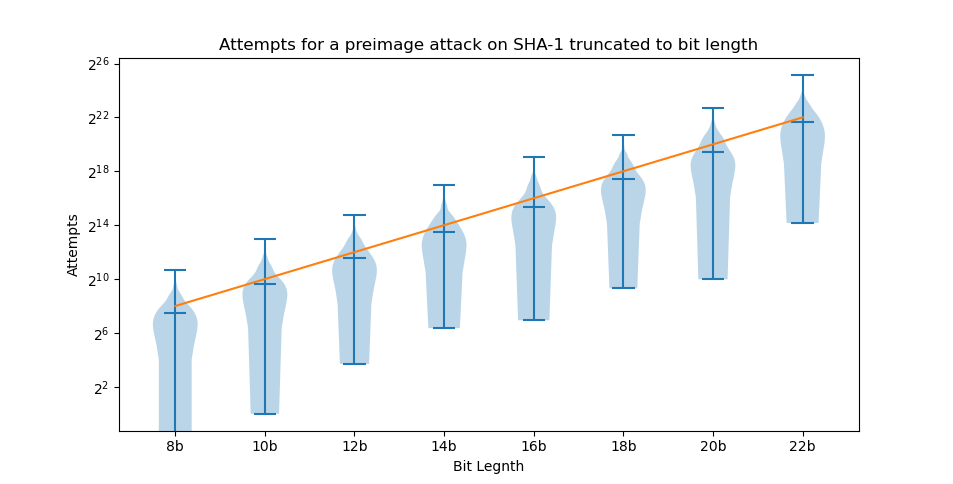
\includegraphics[width=.9\linewidth]{preimage.png}
\end{center}

As we can see in the chart above the number of iterations required scales exponentially (keeping in mind that the Y-axis is logarithmic). This is because with each bit we add to the output digest we double the search space. The expected results closely match my experimentally calculated results, with the violin plot showing where the distribution of samples lies.
\section*{Collision Attach}
\label{sec:org8e9388b}
For a collision attack we make the overall task much easier, the only goal here for attackers is to find any two messages that produce the same output. Additionally, instead of throwing away work as we did in the second preimage attack, we can keep all previously calculated hashes to check our newly generated hashes against.

\begin{center}
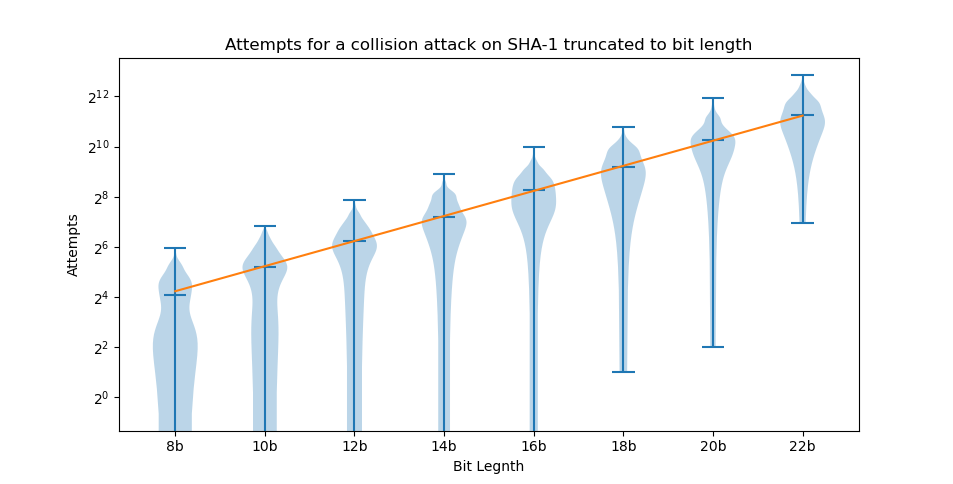
\includegraphics[width=.9\linewidth]{collision.png}
\end{center}

This time we can see that the overall number of attempts required is much lower than in the second preimage attack. Additionally, my results once again closely following the expected number of iterations needed to find a collision.
\section*{Peer Review}
\label{sec:orgb9b20c3}
Chris White was able to review my report.
\end{document}
